\documentclass{article}
\usepackage[utf8]{inputenc}
\usepackage[T1]{fontenc}
\usepackage{graphicx}
\usepackage{hyperref}
\usepackage{geometry}
\geometry{margin=1in}

\title{CAVPANUS}
\date{Encyclopaedia Britannica (1771)}

\begin{document}
\maketitle

\section*{Historical source}
\textbf{Entry ID:} \texttt{entry-cavpanus-1670} \\
\textbf{Volume ID:} 149978642 \\
\textbf{Character Count:} 2269

\subsection*{Extracted Text}
CAVPANUS, a must give by force authors to a woman that adhere to and grows the bottoms of flips to which it is extremely pericious, especially in the East and Well states to prevent this, several dips have intact been themed with copper, to the first trial of which was made on his majelly's firegate the Alarm. CAMPAIS, in fortany. Y. a genus of the monos- gyria order, belonging to the polyamidefs chaf of plants : and in the natural method making under the aitho des, Plantainies. The only is terapylish and ceri-scous three petals are four; the luminous arm long; the fruit is a berty, common, molecular, and podunca-lated, or furnished with a root fluid.

There are fewen species. The fininois, or com- mon copy, is a low limb, generally growing out of the joints of old walls, the lifters of rocks, and a- monglet rabbi, in most of the warm parts of Europe : is in such very little, which lend out many lateral flex- der branches; a matter of that the picked two short crooked liniers, between which and the branches come out the fourth of the leaves, which are single, floors, and Indians around smooth entire list. At letter-mediate joints, between the branches, come out the flower on long footballs, before there endward, the bud with the equipment is gathered for pickling. Thief which are left expand in front of a fingro rofs, having five large white points, which are overall and canvary in the middle are placed a great number of long flaminas, surrounding a flyk which rifles above thing, and crowned with an runn germs, which afterwards because our visible filled with kidney-shaped feeds.

Cultures. This plant is very differently preferred in Britain; it ddigits to grow in creviices of rocks, old walks. Ke and always thrive built its an honourous pu- fiure, is that when planted either in pots on in the full ground, they felddon thrive, though they may be kept alive for home years. They are propagated by foods in the warm parts of Europe, but very feldon in Britain.

\_Ofre. The buds, picked with vinegar, Sez are brought to Britain annually from Italy and the Medi-terranean. They are fuppoted to excite appetite and still life projections, and to be particularly fertile a deter- gents and appraiser in individualities of the liver and fpteen.



\section*{Source record}
\begin{itemize}
\item \textbf{Dataset:} \texttt{NationalLibraryOfScotland/encyclopaedia\_britannica\_illustrated}
\item \textbf{Dataset Revision:} \texttt{309f765b1ecc83e0a7f7762e44b4a927a7555443}
\item \textbf{Page ID:} \texttt{britannica:309f765b1ecc83e0a7f7762e44b4a927a7555443:train:1670} \\
  \textbf{Filename:} \texttt{page-1670-ced69857efba.jpg} \\
  \textbf{Row Index:} 1670 \\
  \textbf{SHA256:} \texttt{ced69857efbaddd7...}
\end{itemize}

\begin{figure}[h]
\centering
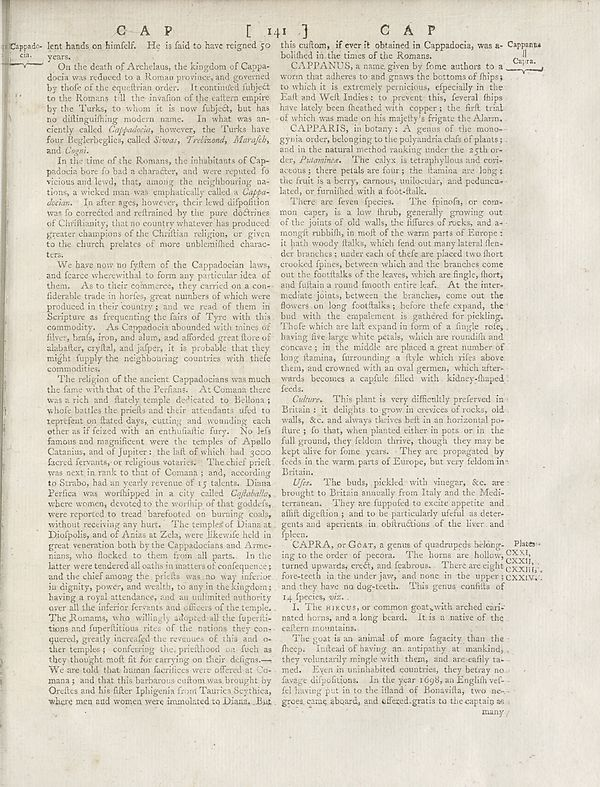
\includegraphics[width=0.85\textwidth]{../scans/page-1670-ced69857efba.jpg}
\caption*{Source scan: \texttt{page-1670-ced69857efba.jpg}}
\end{figure}

\end{document}
